\documentclass{report}
\usepackage{float}

% depricated
\title{
	\iffalse
	\begin{tikzpicture}[remember picture,overlay]
		\node[anchor=north west,yshift=-5pt,xshift=-200pt]%
		at (current page.north east)
		{
\includegraphics[height=30mm]{unitn-logo}};
	\end{tikzpicture}
	\huge 
	\fi
	Fix Mi \\
	Analisi dei Requisiti
}
\author{Giovanni Santini, Riginel Ungureanu, Valerio Asaro}
\date{Anno accademico 2023/2024}

% for the image in the title
\usepackage{tikz}

% custom spacing
\usepackage{setspace}
\onehalfspacing

% footer and header
\usepackage{fancyhdr}
% \setlength{\headheight}{15.2pt}

% Table of contents link to corresponding sections
\usepackage{hyperref}
\hypersetup{
	colorlinks,
	citecolor=black,
	filecolor=black,
	linkcolor=black,
	urlcolor=black
}

\usepackage{amsmath}
% Remove che "Chapter" string before chapters
\iffalse
\makeatletter
\def\@makechapterhead#1{%
	\vspace*{50\p@}%
	{\parindent \z@ \raggedright \normalfont
		\interlinepenalty\@M
		\Huge\bfseries  \thechapter.\quad #1\par\nobreak
		\vskip 40\p@
}}
\makeatother
\fi

% Fancy chapters
\usepackage[Bjarne]{fncychap}
% options: Sonny, Lenny, Glenn, Conny, Rejne, Bjarne, Bjornstrup

\begin{document}
	
	
	%title page
	\begin{titlepage}
		\begin{figure}[t]
			\centering
\includegraphics[width=0.3\textwidth]{images/unitn-logo}
		\end{figure}
		\begin{center}
			\textsc{ \LARGE{Università degli Studi di Trento \\}}
			\textsc{ \LARGE{Facoltà di Informatica\\ }}
			\textnormal{ \LARGE{Corso di Ingegneria del Software\\}}
			\vspace{30mm}
			\fontsize{10mm}{7mm}\selectfont 
			\textup{Fix Mi \\ Specifica dei Requisiti}\\
		\end{center}
		
		\vspace{25mm}
		
		\centering
		\large Gruppo G43: \\ Giovanni Santini\\ Riginel Ungureanu \\ Valerio Asaro
		
		\vspace{20mm}
		
		\centering{\large{Anno Accademico 2023/2024 \\ Trento }}
		
	\end{titlepage}
	
	
	
	
	% use header and footers
	\pagestyle{fancy}
	\fancyhead[R]{\chaptername\ \thechapter}  % header
	
	%\maketitle
	\tableofcontents
	\newpage
	
	
	
	\section{Scopo del documento}
	
	Nel presente documento vengono riportate le specifiche dei requisiti di sistema del progetto FixMi,  attraverso diagrammi di tipo Unified Modeling Language (UML) e tabelle strutturate.\\
	
	
	
	\section{Informazioni del Documento}
	
	% table
	\begin{center} % center the table
		\centering
		\begin{tabular}{ |p{4cm}|p{4cm}|  }
			\hline
			\centering Campo & \qquad\qquad Valore \\ % I found no other way...
			\hline
			Titolo del Documento & Specifica dei Requisiti \\
			\hline
			Titolo del Progetto & Fix Mi \\
			\hline
			Autori del Documento &
			Giovanni Santini \\ & Riginel Ungureanu \\ & Valerio Asaro \\
			\hline
			Amministratore Progetto & Riginel Ungureanu\\
			\hline
			Versione del documento & 1.0 \\
			\hline
		\end{tabular}
	\end{center}


\chapter{Requisiti}

	
\section{Requisiti Funzionali}

\begin{itemize}
	\item Use Case Diagram: Visione esterna del sistema
	\item Sequence Diagram: Rappresenta come gli oggetti collaborano
	\item State Machine Diagram: Stati e Transizioni
	\item Activity Diagram: Attività che innescano altre attività (tasks)
	\item Spiegazione in italiano (da mettere sempre)
\end{itemize}

\subsection*{RF1 Login }
\begin{figure}[H]
	\centering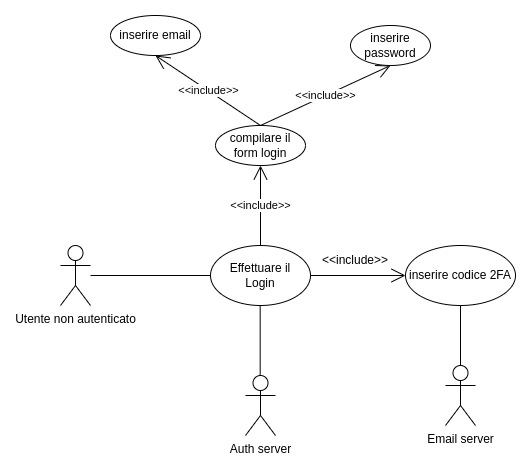
\includegraphics[width=1\textwidth]{images/Login_UCD.drawio.png}
	Use Case Diagram  del login
\end{figure}
Per descrivere questo use case, facciamo uso di un diagramma delle attività swimlane:
\begin{figure}[H]
	\centering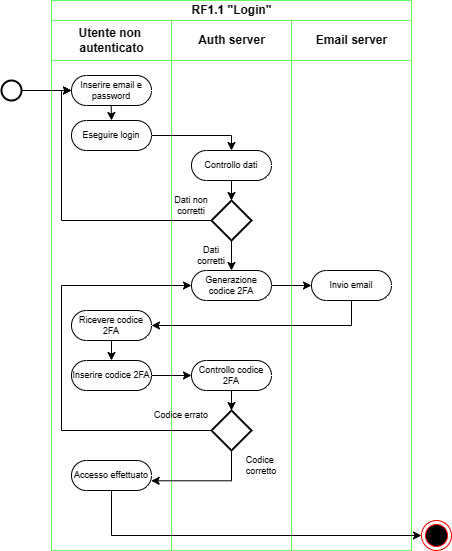
\includegraphics[width=1\textwidth]{images/Login_Swimlane.drawio.png}
	diagramma delle Attività swimlane del Login
\end{figure}
\subsection*{RF2 Registrazione}
\begin{figure}[H]
	\centering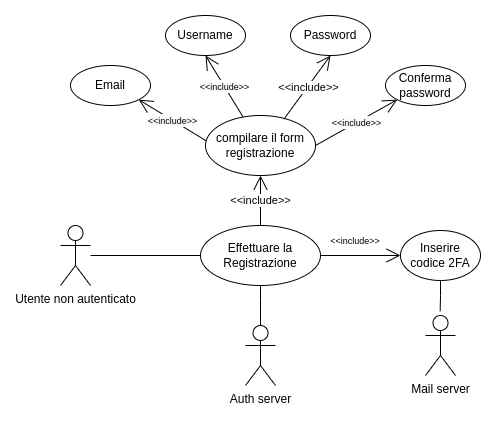
\includegraphics[width=1\textwidth]{images/Registrazione_UCD.drawio.png}
	Use Case Diagram  della registrazione
\end{figure}
Per descrivere questo use case, facciamo uso di un diagramma delle attività swimlane:
\begin{figure}[H]
	\centering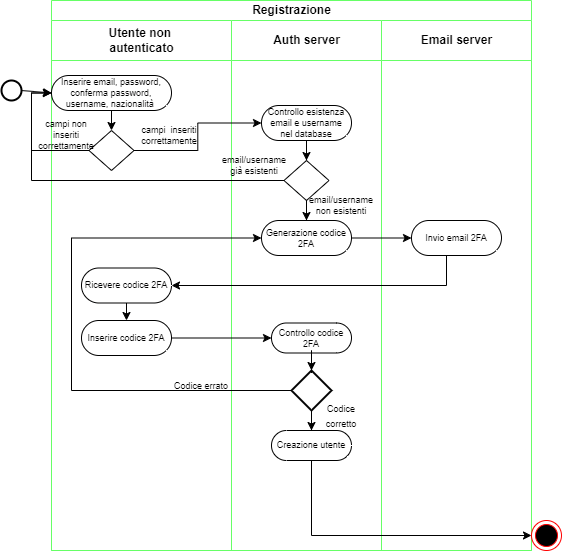
\includegraphics[width=1\textwidth]{images/Register_swimlane.drawio.png}
	diagramma delle Attività swimlane della registrazione
\end{figure}

\subsection*{RF4 Informazioni /  Contatti}

\begin{figure}[H]
	\centering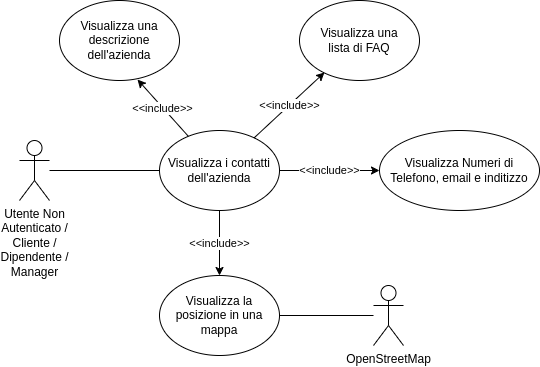
\includegraphics[width=1\textwidth]{images/contatti_sequence_diagram.png}
\end{figure}


\subsection*{RF3 Negozio utente non autenticato + RF5 Negozio utente autenticato}

\begin{figure}[H]
	\centering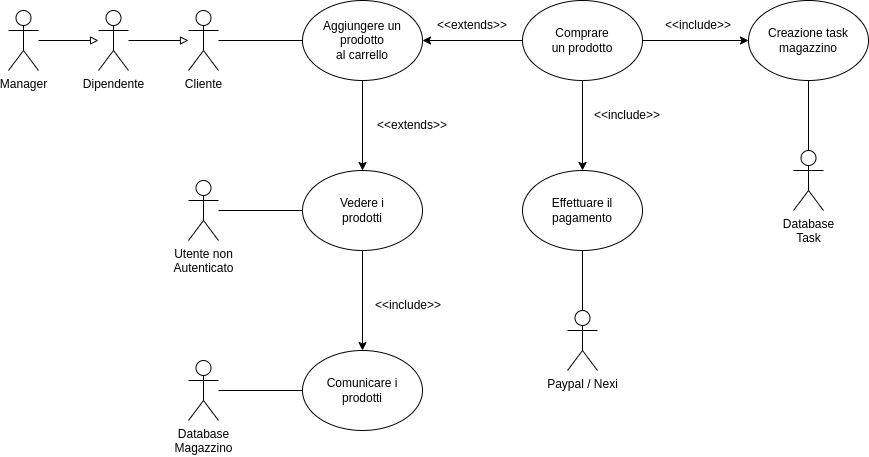
\includegraphics[width=1\textwidth]{images/shop_diagram_1.png}
\end{figure}

\begin{figure}[H]
	\centering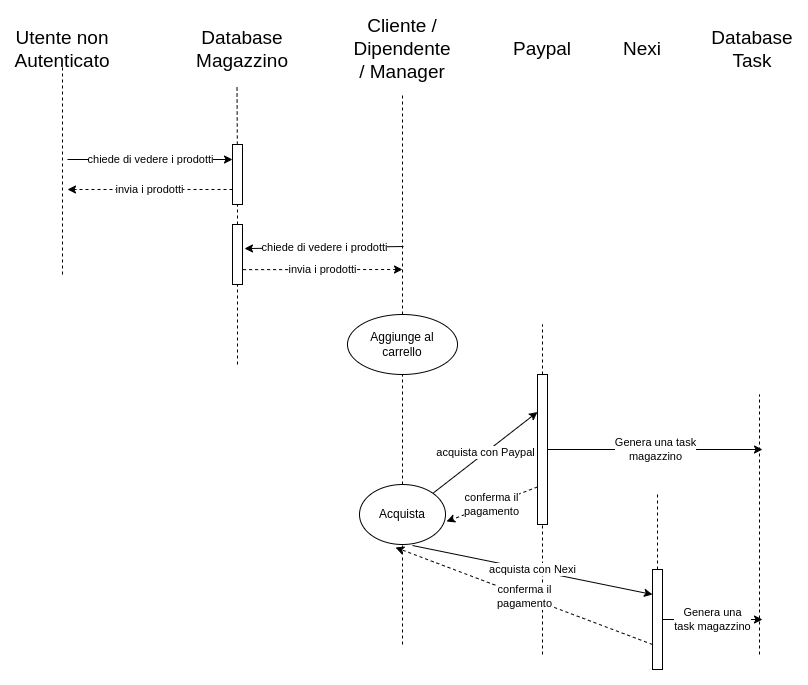
\includegraphics[width=1\textwidth]{images/negozio_sequence_diagram.png}
	diagramma delle Attività swimlane della registrazione
\end{figure}

\subsection*{RF6 Riparazione}
\begin{figure}[H]
	\centering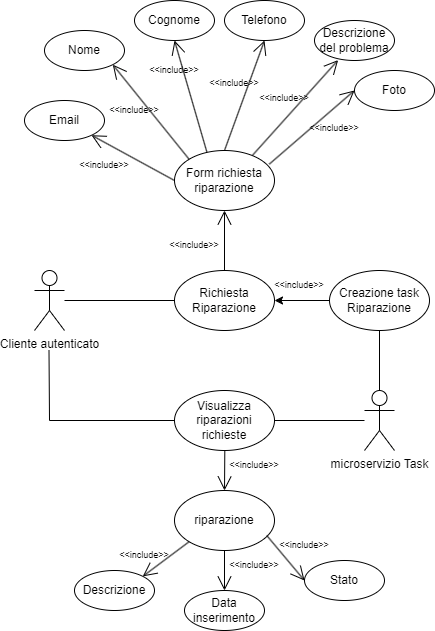
\includegraphics[width=1\textwidth]{images/Riparazione_UCD.drawio.png}
	Use Case Diagram  della riparazione
\end{figure}
\subsubsection*{Descrizione Use Case "Riparazione"}
\textbf{Titolo}: Riparazione \newline
\textbf{Riassunto}: Questo use case descrive come un utente può richiedere una riparazione e visualizzarne lo stato. \newline
\textbf{Descrizione}:
	\begin{enumerate}
		\item L'utente autenticato seleziona la pagina "Riparazioni";
		\item Il sito mostra lo stato delle riparazioni già richieste dall'utente [Exception 1];
		\item Il sito mostra un form per richiedere una nuova riparazione con i seguenti campi:
		\begin{itemize}
			\item nome[Exception 2];
			\item cognome[Exception 2]; 
			\item e-mail[Exception 2];
			\item numero di telefono[Exception 2];
			\item descrizione del problema[Exception 2];
			\item foto (( facoltativo ));
		\end{itemize}
		\item L'utente, appena compilato il form, può inviarlo premendo l'apposito pulsante;
		\item Il sistema, appena ricevuta la richiesta di riparazione, la inserisce nel sistema delle task come "task riparazione";
		
	\end{enumerate}
\textbf{Exceptions}
\begin{itemize}
	\item {[Exception 1]}: Se L'utente non ha nessuna riparazione richiesta, l'elenco sarà vuoto;
	\item {[ Exception 2]}: Se l'utente non ha compilato i campi "nome","cognome","e-mail","numero di telefono","descrizione del problema" non può inviare la richiesta;
\end{itemize}
\subsection*{RF7 Assistenza}

\begin{figure}[H]
	\centering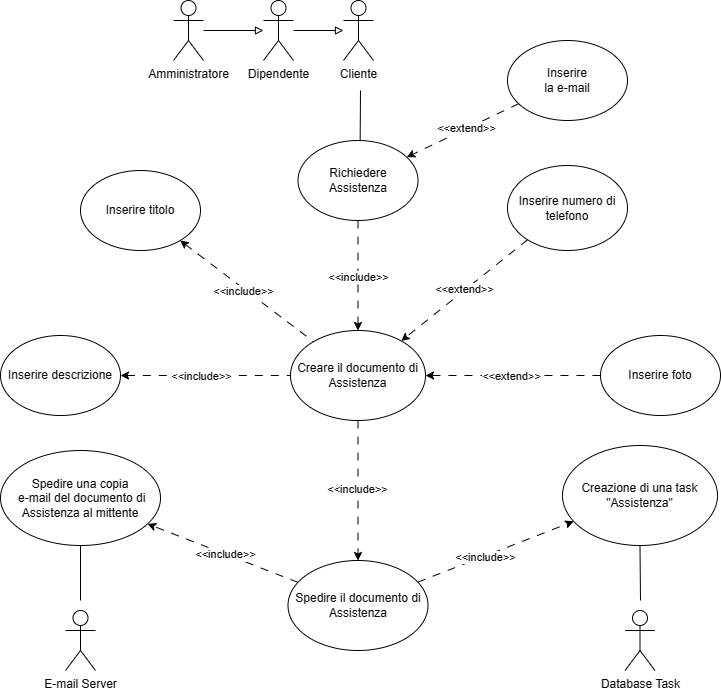
\includegraphics[width=1\textwidth]{images/RF7_assistenza_UCD.png}
\end{figure}


\subsection*{RF8 Feedback}

\begin{figure}[H]
	\centering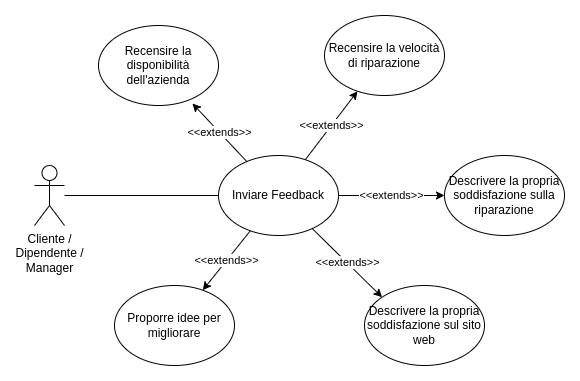
\includegraphics[width=0.9\textwidth]{images/feedback_UCD.png}
\end{figure}

\subsection*{RF9 Tasks}

\subsection*{RF10 Magazzino}
\begin{figure}[H]
	\centering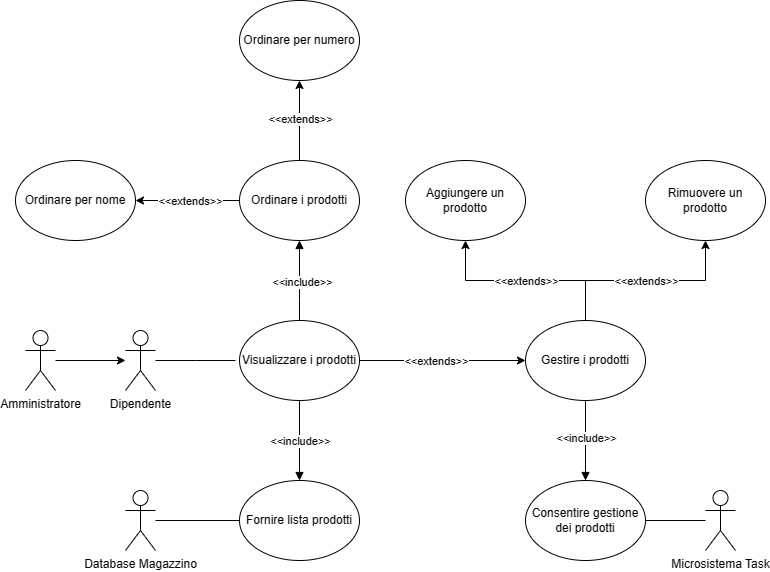
\includegraphics[width=1\textwidth]{images/magazzino_UCD.png}
\end{figure}


\subsection*{RF11 Gestione Dipendenti}


\begin{figure}[H]


\centering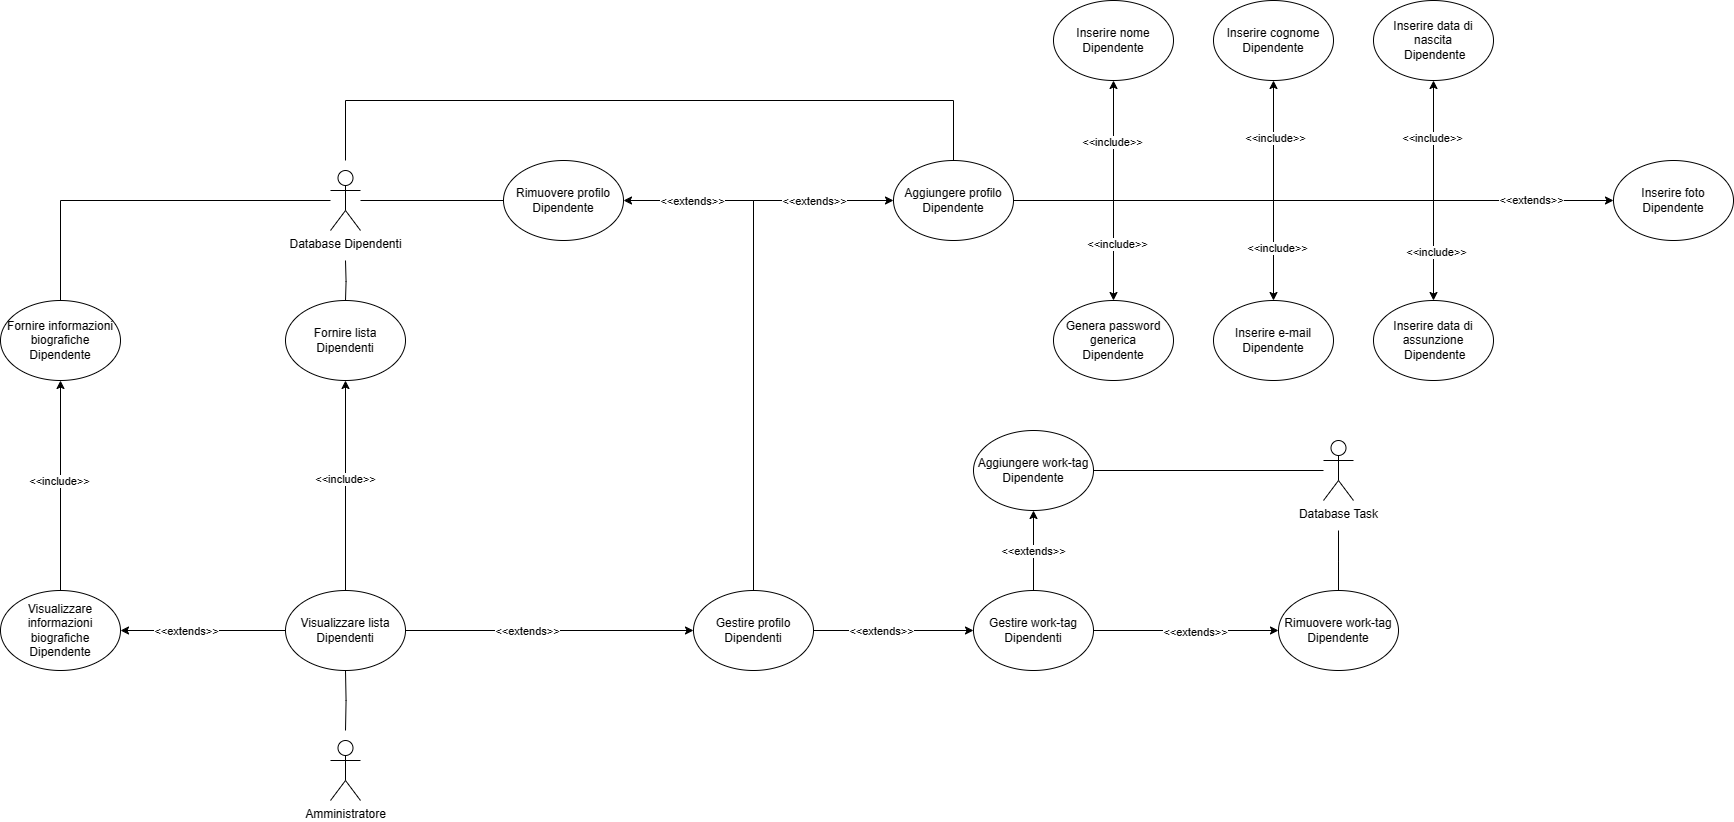
\includegraphics[width=1\textwidth]{images/gestione_dipendenti_UCD.png}  % Non riesco a fare in modo che l'immagine si veda abbastanza grande, probabilmente il grafico stesso è troppo grande.....lo aggiusterò in seguito....credo....probabilmente c'ò solo da posizionare gli elementi in maniera corretta....
\end{figure}
\pagebreak

\section{Requisiti Non Funzionali}
Nel seguente capitolo vengono riportati i requisiti non funzionali (RNF) del sistema utilizzando tabelle strutturate e specificando misure facilmente misurabili


\subsection*{RNF1 Intuitività e Accessibilità}
% table
\begin{center} % center the table
	\centering
	\begin{tabular}{ |p{3cm}|p{4cm}|p{4cm}|  }
		\hline
		\centering Proprietà & \qquad\quad Descrizione & \qquad\qquad Misura\\ % I found no other way...
		\hline
		Linguaggio Comprensibile & In media l’utente deve essere in grado di capire le funzionalità dell'applicazione con una
		sola lettura della descrizione. & In media, il numero di click errati che l'utente compie deve essere minore di 4. \\
		\hline
		Presenza della lingua Inglese e Italiana & Il sito presenta sia la lingua Italiana che quella Inglese, l'utente con un livello di lingua "A1" è in grado di leggere e comprendere il contenuto. & La scelta del vocabolario linguistico utilizzato è conforme con il vocabolario Italiano di livello A1 e Inglese livello A1.\\ % I found no other way...
		\hline
		Consistenza & Il sito deve avere un design consistente, utilizzando un singolo font e una palette fissa di colori. & numero di font utilizzati uguale a 1, numero di colori utilizzati minore di 6.  \\% I found no other way... 
		\hline
	\end{tabular}
\end{center}

\subsection*{RNF2 Sicurezza}
% table
\begin{center} % center the table
	\centering
	\begin{tabular}{ |p{3cm}|p{4cm}|p{4cm}|  }
		\hline
		\centering Proprietà & \qquad\quad Descrizione & \qquad\qquad Misura\\ % I found no other way...
		\hline
		Protezione dati & Il sito deve proteggere i dati sensibili utilizzando un algoritmo di hashing "SHA-3" per sarlvare e controllare le password e protocolli tls e https per ogni comunicazione tra utenti e servizi. & L'applicazione utilizza un algoritmo di hashing "SHA-3" nel salvataggio e controllo di password nel database e utilizza protocolli "tls" e "https" per ogni comunicazione tra utenti e servizi.\\
		\hline
		2 Factor Authentication (2FA) & Il sito deve verificare l'identità dell'utente attraverso il 2FA. & Impossibilità di accedere al sito senza 2FA.\\
		\hline
		Conformità password & La password di un utente deve avere una lunghezza minima di 10 caratteri e deve presentare almeno un numero,una lettera maiuscola, e un carattere speciale. &
		numero dei caratteri maggiore di nove, presenza di almeno un numero,lettera maiuscola e carattere speciala dalla seguente lista:		\begin{verbatim} ! ? $ % ^ & * ( ) _ \end{verbatim} \begin{verbatim}- + = { [ } ] : ;\end{verbatim} \begin{verbatim}@ # | \ < , > . \end{verbatim} \\
		\hline
		
	\end{tabular}
\end{center}
\subsection*{RNF3 Privacy}
% table
\begin{center} % center the table
	\centering
	\begin{tabular}{ |p{3cm}|p{4cm}|p{4cm}|  }
		\hline
		\centering Proprietà & \qquad\quad Descrizione & \qquad\qquad Misura\\ % I found no other way...
		\hline
		GDPR & il sito deve essere conforme alle principali direttive del GDPR, tra cui il consenso esplicito per la raccolta dei dati, la trasparenza nell'uso dei dati, la possibilità di accesso e cancellazione dei dati personali da parte dell'individuo, e misure di sicurezza per proteggere tali dati & Conforme \\
		\hline
	\end{tabular}
\end{center}
\subsection*{RNF4 Affidabilità e Disponibilità}
% table
\begin{center} % center the table
	\centering
	\begin{tabular}{ |p{3cm}|p{4cm}|p{4cm}|  }
		\hline
		\centering Proprietà & \qquad\quad Descrizione & \qquad\qquad Misura\\ % I found no other way...
		\hline
		Risultati desiderati & La probabilità che il sito fornisca i risultati desiderati senza interruzioni o tempi di inattività deve essere maggiore del 99\% (novantanove percento) & $\frac{\text{risultati ricevuti con successo}}{\text{risultati totali}} $ \\ % There was no other way...
		\hline
		Operatività &  la probabilità che il sito rimanga operativo in un determinato momento
		indipendentemente dal numero di guasti già subiti dal sistema deve essere maggiore del 99\% (novantanove percento) & $ \frac{\text{secondi di attività dal lancio}}{\text{secondi totali dal lancio}} $\\
		\hline 
	\end{tabular}
\end{center}
\subsection*{RNF5 Performante}
% table
\begin{center} % center the table
	\centering
	\begin{tabular}{ |p{3cm}|p{4cm}|p{4cm}|  }
		\hline
		\centering Proprietà & \qquad\quad Descrizione & \qquad\qquad Misura\\ % I found no other way...
		\hline
		Aggiornamento negozio & Il sito deve aggiornare la lista degli articoli presenti in negozio, in caso di modifica al magazzino, in meno di un secondo. & Secondi \\
		\hline 
		2 Factor Authentication (2FA)& Il sito deve inviare la mail di 2FA in meno di cinque secondi. & Secondi \\
		\hline
		Lista delle Task & Il sito deve aggiornare la lista delle task in meno di un secondo. & Secondi \\ 
		\hline

	\end{tabular}
\end{center}
\subsection*{RNF6 Compatibilità e Portabilità}
% table
\begin{center} % center the table
	\centering
	\begin{tabular}{ |p{3cm}|p{4cm}|p{4cm}|  }
		\hline
		\centering Proprietà & \qquad\quad Descrizione & \qquad\qquad Misura\\ % I found no other way...
		\hline
		Compatibilità dispositivi lato client & L'applicazione lato cliente  deve essere disponibile per dispositivi aventi un browser che supporta \begin{itemize}
		\item html5
		\item https
		\item tls 1.2
		\end{itemize} & \\
		\hline
		Compatibilità dispositivi lato server & L'applicazione lato server deve essere disponibile per computer che supportino: 
		\begin{itemize}
			\item Node js 18.18.0 LTS
			\item MongoDB 7.0
		\end{itemize}
		& \\
		\hline 
		Responsive su TV e monitor di PC e Laptop & Il sito deve potersi adattare alla dimensione degli schermi con Aspect Ratio da 4:3, 16:9, 21:9 & Aspect Ratio \\
		\hline
		Responsive su Smartphone & Il sito deve potersi adattare agli schermi dei seguenti Smartphone: 
		\begin{itemize}
			\item Iphone X,XR,11,\dots , 14
			\item Tutti i modelli Xiaomi dal 2018 in poi 
			\item Tutti i modelli Samsung dal 2018 in poi
			\item Tutti i modelli Motorola dal 2018 in poi 
			\item Tutti i modelli Huawei dal 2018 in poi 
		\end{itemize}
		& \\
		
		\hline
		
	\end{tabular}
\end{center}
\begin{center} % center the table
	\centering
	\begin{tabular}{ |p{3cm}|p{4cm}|p{4cm}|  }
		\hline
		Responsive su Tablet & Il sito deve potersi adattare agli schermi dei seguenti Tablet: 
		\begin{itemize}
			\item Ipad Air, Pro dal 2018 in poi
			\item Tutti i modelli Xiaomi dal 2018 in poi
			\item Tutti i modelli Samsung dal 2018 in poi
		\end{itemize} & \\
		\hline
		
		
	\end{tabular}
\end{center}
\subsection*{RNF7 Mantenibilità e Scalabilità}
% table
\begin{center} % center the table
	\centering
	\begin{tabular}{ |p{3cm}|p{4cm}|p{4cm}|  }
		\hline
		\centering Proprietà & \qquad\quad Descrizione & \qquad\qquad Misura\\ % I found no other way...
		\hline
		Team di manutenzione &  Al sito deve essere affiancato, prima e dopo il rilascio ufficiale, un team di
		manutenzione che si occupi di testare ogni funzionalit`a periodicamente e
		che, su richiesta qualora ci siano problemi, sia pronto a intervenire tempestivamente
		 & \\
		\hline
		sito facilmente mantenibile & Il sito deve possedere le seguenti caratteristiche
		\begin{itemize}
			\item Il codice sorgente del back-end dev'essere modulare, utilizzando un'architetture a microserivizi
			\item Il codice sorgetne deve rispettare le linee guida del linguaggio scelto
		\end{itemize}
		& Conformità Linee guida Javascript
		\\  \hline

	\end{tabular}
\end{center}
\subsection*{RNF8 Conformità}
\begin{center} % center the table
	\centering
	\begin{tabular}{ |p{3cm}|p{4cm}|p{4cm}|  }
		\hline
		\centering Proprietà & \qquad\quad Descrizione & \qquad\qquad Misura\\ % I found no other way...
		\hline
		Conformità leggi & L'applicazione deve essere conforme alle normative di legge in materia di siti web imposti dall'Unione Europea & Conforme \\
		\hline
		Conformità GDPR & L'applicazione deve essere conforme al GDPR, come descritto in RNF3 & Conforme \\
		\hline
		Conformità W3C WAI & L'applicazione deve essere conforme al W3C WAI (Web Accessibility Initiative) & Conforme \\ 
		\hline
	\end{tabular}

\end{center}


\chapter{Analisi del Contesto}

\section{Utenti e Sistemi Esterni}

Sono stati individuati tutti gli Utenti ed i Sistemi Esterni che fanno parte del funzionamento del sistema "Fix Mi".\\Segue una elencazione di ogni elemento con una descrizione breve adibita.


\subsection{Utente}
Con il termine "Utente" si definisce una qualsiasi persona che abbia fatto accesso al sistema senza essersi identificati. L'Utente è in grado di:
\begin{itemize}
	\item Accedere all'area "Negozio" per visualizzare il catalogo.
	\item Accedere all'area "Informazioni / Contatti" e visualizzarne i dettagli. 
	%tutti i dettagli in esso contenuti, tra cui numeri telefonici, indirizzi di posta elettronica e posizione geografica aziendale.
\end{itemize}


\subsection{Cliente}

Con il termine "Cliente" si intende un Utente che abbia compiuto con successo la registrazione nel sistema e che successivamente abbia fatto l'accesso nel suo profilo. Il Cliente, oltre a potere accedere a tutti i servizi offerti ad un profilo "Utente", è in grado di
\begin{itemize}
	\item Inserire gli articoli dell'area "Negozio" nel proprio carrello e, successivamente, effettuarne l'acquisto.
	\item Accedere all'area "Riparazione" per visualizzare la lista di riparazioni in corso, creare una nuova richiesta di Riparazione o eliminarne una esistente.
	%\item Inviare feedback riguardo la qualità dei servizi offerti. (Lmao non ho ancora capito se questo c'è oppure no).
\end{itemize}
\subsection{Dipendente}

Con il termine "Dipendente" si intende quella persona che abbia stipulato un contratto di lavoro con l'azienda. Il Dipendente, oltre a poter usufruire di tutti i servizi adibiti ad un profilo Cliente, può:
\begin{itemize}
	\item Accedere all'area "Magazzino" per visualizzare la lista dei prodotti posseduti, aggiungere un nuovo articolo o rimuoverne uno esistente.
	\item Accedere all'area "Task" per visualizzare la lista delle Task, crearne una nuova, contrassegnarla o rimuoverne una esistente. 
\end{itemize}

\subsection{Manager}

Con il termine "Manager" si intende quella persona che abbia il completo controllo del sistema e dell'azienda. Il Manager, oltre a potere accedere a tutte le aree offerte al profilo Dipendente, è in grado di:
\begin{itemize}
	\item Accedere all'area "Gestione Dipendenti" per visualizzarne la lista, aggiungere un nuovo profilo Dipendente o eliminarne uno esistente.
\end{itemize}

\subsection{Server Mail}
Attraverso la Server Mail, il sistema è in grado di mandare e ricevere e-mail. 

\subsection{Database Autenticazione}
Il database "Autenticazione" ("Auth") memorizza i dati utilizzati a riconoscere i profili creati durante la registrazione nel sistema.
%memorizza i dati utilizzati durante la fase di registrazione di un Utente, controllando che essi non siano già esistenti o errati. In fase di Login tali dati verranno controllati per verificare che l'Utente stia facendo accesso ad un profilo esistente.  (Non sono sicuro di questo ma beh lo lascio qui cosi nel caso per cambiarlo non ci vuole niente)

\subsection{Database Magazzino}
Il database "Magazzino" contiene la lista di prodotti contenuti nel catalogo dell'azienda.

\subsection{Database Task}
Il database "Task" contiene la lista di tutte le task, il loro tag e lo stato.

\subsection{PayPal}
Il servizio esterno "PayPal" permette al Cliente di effettuare acquisti all'interno del sistema.

\subsection{Nexi}
Il servizio esterno "NeXi" permette al Cliente di effettuare acquisti all'interno del sistema.

\subsection{OpenStreetMap}
Il servizio esterno "OpenStreetMap" fornisce dati geografici al sistema.%per visualizzare la posizione aziendale geografica in cartina.

\subsection{2FA}
Il 2FA ("Two Factor Authentication") si occupa di verificare che la e-mail inserita dall'utente in procinto di registrarsi o accedere sia corretta ed esistente.
%In particolare il codice contenuto nel 2FA viene spedito all'indirizzo di posta elettronica inserito dall'Utente che, nel caso sia inesistente, non potrebbe essere visualizzato. (Non sono sicuro se scrivere anche questo o no....)

\subsection{Microservizi}
Autentication Server, Microservizio Task


\section{Diagramma di Contesto}

Spiegare la back-end andando su vari livelli di dettaglio:
\begin{itemize}
	\item Context diagram generale
	\item Divisione in processi
	\item Divisione in Sub Processi
	\item Data flow diagram per i processi (e i sub processi se siamo bravi)
\end{itemize}
\chapter{Analisi dei Componenti}

\section{Definizione dei Componenti}

Componenti interni della mia applicazione e come interagiscono\\
Sostanzialmente sono i componenti usati nei RF in questo documento

\section{Diagramma dei Componenti}

\end{document}